\documentclass[10pt,paper=a4,final]{scrartcl}
\usepackage[utf8]{inputenc}
\usepackage{tabularx}	%used for the tables
\usepackage{geometry}	%allows us to specify the 'seitenrand'
\usepackage[table]{xcolor}	%allows us to make colored fields in the tables
\usepackage{graphicx}	%package used to include graphics
\usepackage{hyperref}   	%used to make klickable links

%\hypersetup{linktocpage}	%make the tableofcontent klickable
\hypersetup{
  colorlinks,
  citecolor=black,
  filecolor=black,
  linkcolor=black,
  urlcolor=black
}

%These two lines will allow us to specify our own headers/footers
\usepackage{fancyhdr}
\pagestyle{fancy}

%The next three lines set the default font to Arial
\usepackage[T1]{fontenc}
\usepackage[scaled]{uarial}
\renewcommand*\familydefault{\sfdefault}


\geometry{a4paper, top=20mm, right=20mm, bottom=20mm, left=20mm}
\title{Konzeptbericht}
\author{Bash Vi, Shylux, Kaleb Tschabolt}
\date{\today}

%defining header and footer
\fancyhf{}	%delete default values
\setlength{\headwidth}{\textwidth}	%header and footer width equal the text width
\fancyhead[LE,LO]{
\includegraphics{header.png}}
\fancyhead[RE,RO]{ProjectExplorer}
\fancyfoot[CE,CO]{Speicherdatum: \today{}}
\fancyfoot[RE,RO]{\thepage}

\begin{document}
\maketitle
\newpage
\begin{tabularx}{\textwidth}{ r X }	%X fields are stretched over the whole space
  \textcolor{white}{{\bf Status}}\cellcolor{blue!80!} & In Arbeit/In Pruefung/{\bf Abgeschlossen}\cellcolor{blue!20!} \\
\textcolor{white}{{\bf Projektname}}\cellcolor{blue!80!} & Projektexplorer\cellcolor{blue!20!} \\
\textcolor{white}{{\bf Projektleiter}}\cellcolor{blue!80!} & Niklaus Hofer\cellcolor{blue!20!} \\
\textcolor{white}{{\bf Auftraggeber}}\cellcolor{blue!80!} & M. Frieden, GIBB\cellcolor{blue!20!} \\
\textcolor{white}{{\bf Autoren}}\cellcolor{blue!80!} & Niklaus Hofer\cellcolor{blue!20!} \\
\textcolor{white}{{\bf Verteiler}}\cellcolor{blue!80!} & Lukas Knoepfel, Kaleb Tschabolt, Niklaus Hofer\cellcolor{blue!20!}
\end{tabularx}
\newline
\newline
\newline
{\bf Aenderungskontrolle, Pruefung, Genehmigung}
\newline

\begin{tabularx}{\textwidth}{l l X X}
\textcolor{white}{Version}\cellcolor{blue!80!} & \textcolor{white}{Datum}\cellcolor{blue!80!} & \textcolor{white}{Beschreibung, Bemerkung}\cellcolor{blue!80!} & \textcolor{white}{Name oder Rolle}\cellcolor{blue!80!} \\
\cellcolor{blue!20!} 0.1 & 22.03.2011 \cellcolor{blue!20!} & Erstellen \cellcolor{blue!20!} & Hofer, Kn\"opfel, Tschabold\cellcolor{blue!20!} \\
\cellcolor{blue!20!} 1.0 & 29.05.2011 \cellcolor{blue!20!} & Verbesserungen, Port nach \LaTeX \cellcolor{blue!20!} & Hofer \cellcolor{blue!20!} \\
\end{tabularx}
\newline
\newline
\newline
{\bf Definitionen und Abkuerzungen}
\newline

\begin{tabularx}{\textwidth}{l X}
\textcolor{white}{Begriff/ Abkuerzung}\cellcolor{blue!80!} & \textcolor{white}{Bedeutung}\cellcolor{blue!80!} \\
\cellcolor{blue!20!} DB & Datenbank \cellcolor{blue!20!} \\
\end{tabularx} 
\newline
\newline
\newline
\bibliographystyle{plain}
\bibliography{konzeptbericht}{}
\flushleft
\newpage
\tableofcontents
\newpage
\section{Zweck des Dokuments}
Zusammenfassung der Ergebnisse der Phase „Konzept“.
\section{Geschäftsprozesse}
Da unser Programm einen sehr generellen Zweck hat und nicht f\"ur eine bestimmte Arbeitsumgebung optimiert ist, gibt es hier keinen Gesch\"aftsprozess der konret beschrieben werde k\"onnte.\\

Um die Einfachheit, und trotzdem die Bedeutung die dem Aufgabengebiet anzumessen ist aufzuzeigen haben wir aber ein Diagram, dass den (im Grunde sehr einfachen) Ablauf der zur \"Offnung einer Datei n\"otig ist aufzeigt.\\
Besonders da dieser Ablauf in einem Arbeitsalltag vielemale wiederholt wird kann durch die Optimierung dessen viel Zeit gewonnen und Frustration verhindert werden.
\begin{figure}[h!]
   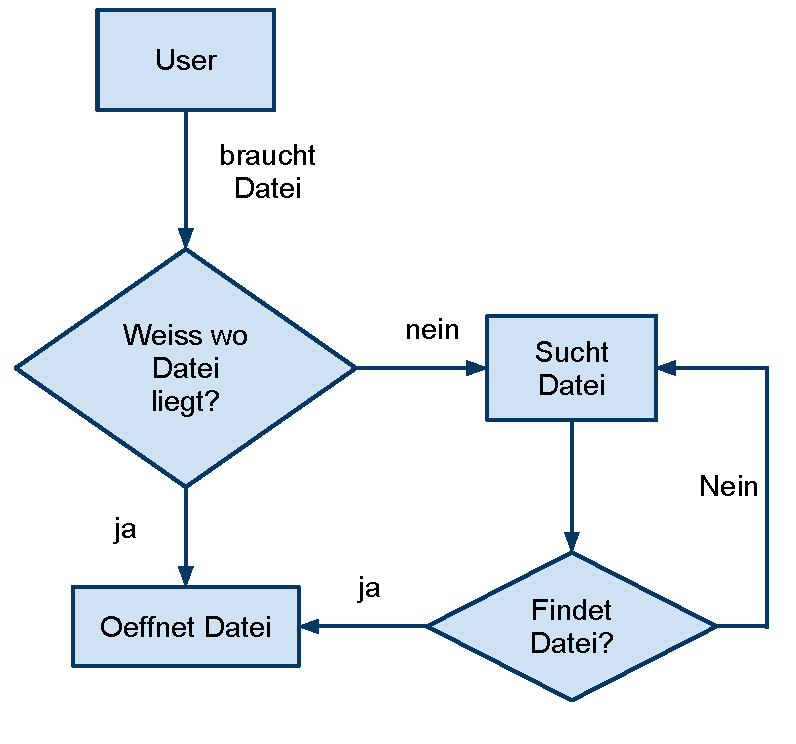
\includegraphics[width = \textwidth]{arbeitsablauf.pdf}
   \caption{Arbeitsablauf beim \"Offnen einer Datei}
  %\label{fin verhindert werden.
\end{figure}


\section{Systemanforderungen}
\subsection{Anforderungen an die Funktionalität}

\subsubsection{Funktionen}
\begin{enumerate}
	\item Dateien verwalten
	\item Allgemein
	\begin{enumerate}
		\item Dateien verschieben, kopieren, löschen
		\item Dateien per Doppelklick \"offnen
		\item Datei-Eigenschaften anzeigen
		\begin{enumerate}
			\item Gr\"osse
			\item Erstelldatum
			\item Zugriffsrechte
			\item zuletzt ge\"offnet
			\item der Datei zugeordnete Tags
		\end{enumerate}
		\item Obige Punkte k\"onnen \"uber ein drop-down erreicht werden, welches wiederum durch Rechtsklick auf eine Datei ge\"offnet wird.
		\item re-read erzwingen - zwingt das Programm die effektiven Datei-Daten von der Festplatte zu lesen und die Datenbank zu aktualisieren.
		\item Ansicht zwischen hierarchisch und tag-view wechseln.
		\item Link zur Datenbank anzeigen
		\item anzeigen alter Dateiversionen (falls backup eingeschaltet ist)
		\item Drag ‘n’ drop von Dateien/Ordnern in andere Ordner und aus den standard Dateimanagern der Systeme.
	\end{enumerate}
	\item Hierarchische Ansicht
	\begin{enumerate}
		\item Dateisystem-Struktur in einer Baumstruktur anzeigen (\"ahnlich wie in Microsoft Windows Explorer)
		\item Einen bestimmten Ordner anhand seiner URL direkt \"offnen
	\end{enumerate}
	\item Tag-view
	\begin{enumerate}
		\item Alle Dateien mit einem bestimmten Tag anzeigen
		\item Alle Dateien mit einem bestimmten Tag innerhalb eines Ordners (reqursiv) anzeigen.
		\item Alle Dateien eines bestimmten Tags \"offnen
		\item Alle Dateien eines bestimmten Tags kopieren (z.B. zur Sicherung)
		\item Tag umbenennen
	\end{enumerate}
	\item Archivierung
	\begin{enumerate}
		\item Kann f\"ur das ganze Dateisystem eingeschalten werden
		\begin{enumerate}
			\item funktioniert aber natuerlich nur bei Dateien f\"ur die der User die n\"otigen Zugriffsrechte hat
			\item Warnung bei auswahl grosser Gesamtgrösse (500MB?).
			\item Warnung bei auswahl von Logfiles (viele modifikationen = viele backups).
		\end{enumerate}
		\item Kann f\"ur einzelne Ordner/ Dateien ein/ausgeschalten werden.
		\item Bei jeder \"Anderung wird eine Kopie der Datei in einem verschtekten Ordner abgelegt. Der Name der Datei wird dabei um die exakten Datum/Zeit Angaben erg\"anzt.
		\item Will der User sp\"ater eine historische Version der Datei ansehen, so kann er dies \"uber die Maske ‘historische Versionen’ die \"uber den Rechtsklick-Dialog der Datei erreicht wird.
		\item L\"oschen aller historischer Versionen einer Datei
		\item L\"oschen aller historischer Versionen aller Dateien eines Ordners (reqursiv)
		\item Ob historische Versionen beim L\"oschen einer Datei auch gel\"oscht werden sollen kann in den Programmeinstellungen festgelegt werden.
	\end{enumerate}
\end{enumerate}
\newpage
\subsubsection{Usecases}
\subsection{Bemerkungen}
\begin{itemize}
	\item F\"ur das Anzeigen der hierarchischen Struktur der Verzeichnisse und Dateien haben wir hier keinen Usecase beschrieben, da dieser Vorgang wohlbekannt und f\"ur viele User Alltag ist.
	\item Dasselbe gilt f\"ur die Dateioperationen (z.B. kopieren, verschieben, …)
\end{itemize}
\begin{figure}[h!]
    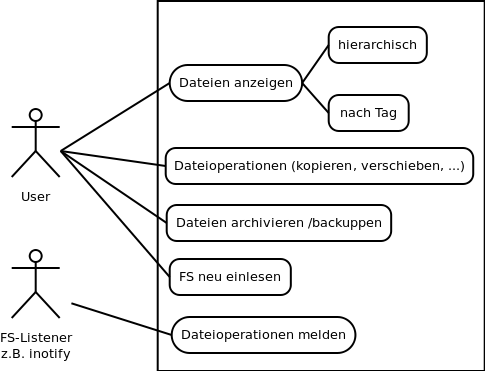
\includegraphics[scale=0.5]{usecases.png}
    \caption{Usecases}
\end{figure}

\begin{tabularx}{\textwidth}{|l|X|}
\hline
\bf Name & {\bf Dateien anzeigen; nach Tag} \\ \hline
Kurzbeschreibung & 	Alle Dateien eines Tags anzeigen \\ \hline
Akteur(e) & User \\ \hline
Ergebniss(e) & 	\begin{itemize}
	\item Alle Dateien die mit dem Tag versehen sind werden angezeigt.
	\item Alle Dateien die mit einem Tag versehen sind und sich innerhalb eines bestimmten Ordners befinden werden angezeigt.
\end{itemize} \\ \hline
Eingehende Daten & Benutzeraktionen \\ \hline
Vorbedingungen & Das Tag muss vorhanden sein. Dem Tag m\"ussen Dateien zugeordnet sein. \\ \hline
Nachbedingungen & Alle Dateien die mit dem Tag versehen wurden werden angezeigt. \\ \hline
Essenzielle Schritte & \begin{enumerate}
	\item Bei Agieren aus der Tag-View
	\begin{enumerate}
		\item Auswahl des gew\"unschten Tags aus der Liste der vorhandenen Tags.
		\begin{enumerate}
			\item Dateien werden jetzt angezeigt
		\end{enumerate}
		\item Auswahl eines Filters
		\begin{enumerate}
			\item Filter nach Ordner
			\item Gew\"unschten Ordner ausw\"ahlen
			\item Dateien des gew\"unschten Tags die sich im gew\"ahlten Ordner (oder einem Unterordner dieses) befinden werden nun angezeigt
		\end{enumerate}
	\end{enumerate}
	\item Bei Agieren aus Hierarchical-View
	\begin{enumerate}
		\item Navigieren zum entsprechenden Ordner.
		\item Rechtsklick; Dateien eines Tags anzeigen; Tag w\"ahlen
		\item Die Ansicht wechselt jetzt automatisch zur Tag-View und Dateien des gew\"unschten Tags die sich im gew\"ahlten Ordner (oder einem Unterordner dieses) befinden werden nun angezeigt.
	\end{enumerate}
\end{enumerate} \\ \hline
Offene Punkte & Es ist noch zu kl\"aren ob auch weitere Filter als nach Ordner zur Verf\"ugung stehen sollen (z.B. Datumsbereich). \\ \hline
\"Anderungshistorie &  22.03.2011; Lukas Knöpfel; Final \\ \hline
\end{tabularx}
\begin{tabularx}{\textwidth}{|l|X|}
\hline
\bf Name		& {\bf Archivierung (archivierte Datei ansehen)} \\ \hline
Kurzbeschreibung	& Die historische Version eines Dokumentes wird angezeigt \\ \hline
Akteur(e)		& User \\ \hline
Ausl\"oser		& \begin{itemize}
  \item In einer alten Version eines Dokumentes wurde etwas gelöscht von dem speter bemerkt wird dass es doch noch benötigt wird.
  \item Die aktuelle Version eines Dokumentes wird mit einer älteren verglichen. \end{itemize} \\ \hline
Ergebniss(e)		& Eine alte Version einer Datei wird geöffnet. \\ \hline
Eingehende Daten	& Benutzeraktionen \\ \hline
Vorbedingungen		& \begin{itemize}
  \item Die entsprechende Datei muss zur Archivierung markiert sein.
  \item Es müssen archivierte Versionen der Datei vorhanden sein. \end{itemize} \\ \hline
Nachbedingungen		& Eine historische Version der Datei ist geöffnet. \\ \hline
Essenzielle Schritte	& \begin{enumerate}
  \item Navigieren zur Datei.
  \item Rechtsklick; Historische Versionen anzeigen.
  \item Eine neue Maske öffnet sich in der alle historischen Versionen der Datei zusammen mit dem Datum an dem die Datei archiviert wurde angezeigt werden.
  \item Ein Doppelklick auf die entsprechende Datei öffnet diese. \end{enumerate} \\ \hline
Offene Punkte		& Werden in der alten Version der Datei änderungen vorgenommen, wohin werden diese dann gespeichert?
Evtl. könnten alte Versionen einer Datei auch als ‘read only’ zur Verfuegung stehen. \\ \hline
Bemerkungen		& In der Maske die die historischen Versionen anzeigt, befindet sich neben jeder Version ein Button, mit dessen Hilfe sich die historische Version wiederherstellen lässt.
Dadurch wird die aktuelle Version archiviert und durch die archivierte überschrieben. \\ \hline
\"Anderungshistorie	& \begin{itemize}
  \item 20.03.2011; Niklaus Hofer; WIP
  \item 28.05.2011; Niklaus Hofer; finished \end{itemize} \\ \hline
\end{tabularx}
\begin{tabularx}{\textwidth}{|l|X|}
\hline
\bf Name		& {\bf FS neu einlesen; Systemdaten einlesen} \\ \hline
Kurzbeschreibung	& Falls von einem externen Programm Dateisystem Operationen ausgeführt werden (z.B. verschieben einer Datei, Umebenennen einer Datei\ldots) während unser Programm nicht läuft bemerkt das unser Programm nicht.
Das kann zu ghost-files (Dateien die im Programm erscheinen, auf FS-Ebene aber nicht erscheinen) führen.
Um das möglichst zu verhindern liest das Programm bei jedem Start die Daten vom Dateisystem ein und gleicht diese mit denen in der Datenbank ab.
Der User kann aber auch zur Laufzeit manuell ein Neueinlesen der Daten anfordern. \\ \hline
Akteur(e)		& User \\ \hline
Ausl\"oser		& Eine Datei die innerhalb des Programms noch erscheint kann nicht mehr geöffnet werden da sie auf FS Ebene nicht mehr verfügbar ist. \\ \hline
Ergebniss(e)		& Das Programm bemerkt das Nichtvorhandensein der Datei und zeigt diese nicht mehr an. \\ \hline
Eingehende Daten	& Benutzeraktionen. Struktur des Dateisystems. \\ \hline
Vorbedingungen		& \begin{itemize}
  \item Eine vom Programm überwachte Datei wurde verschoben.
  \item Die Aktion wurde von Programm nicht bemerkt. \end{itemize} \\ \hline
Nachbedingungen		& Innerhalb des Programs wird die nicht mehr existente Datei nicht mehr angezeigt. \\ \hline
Essenzielle Schritte	& \begin{enumerate}
  \item In der Menuleiste wird der Eintrag Program; Neueinlesen des Dateisystems gewählt. \begin{enumerate}
      \item Nun kann ausgewählt werden zwischen dem Aktualisieren aller überwachten Verzeichnisse und dem Aktualisieren bloss eines einzelnen Verzeichnisses (reqursiv). \end{enumerate} \end{enumerate}\\ \hline
Bemerkungen		& Dieser Vorgang wird auch bei jedem Neustart des Programmes ausgeführt. \\ \hline
\"Anderungshistorie	& \begin{itemize}
  \item 20.03.2011; Niklaus Hofer; WIP
  \item 28.05.2011; Niklaus Hofer; finished \end{itemize} \\ \hline
\end{tabularx}
\begin{tabularx}{\textwidth}{|l|X|}
\hline
\bf Name		& {\bf Dateioperationen melden} \\ \hline
Kurzbeschreibung	& Eine Datei wird ausserhalb des Programmes verschoben währen dieses läuft. \\ \hline
Akteur(e)		& User \\ \hline
Ausl\"oser		& Eine Datei wird mit einem anderen Programm (z.B. mv, Windows Explorer, …) verschoben oder kopiert. \\ \hline
Ergebniss(e)		& Das Programm wird über die Aktion informiert und kann die Datenbank anpassen. \\ \hline
Eingehende Daten	& Information über die Aktion durch einen FS-Listener. \\ \hline
Vorbedingungen		& \begin{itemize}
  \item Die Datei die verschoben/ kopiert/ gelöscht wird muss in einem überwachten Ordner liegen.
  \item Das Programm muss laufen. \end{itemize} \\ \hline
Nachbedingungen		& Der Datenbankeintrag der entsprechenden Datei wurde automatisch angepasst.
Falls die Datei kopiert wurde, so hat die neue Kopie dieselben Tags wie die alte Version.
Sollte die Datei gelöscht werden und für die Archivierung markiert sein so wird sie zuvor noch in den Ordner mit den Archiven kopiert.\\ \hline
Essenzielle Schritte	& \begin{enumerate}
  \item Der Nutzer löst die Aktion aus indem er ausserhalb des Programmes eine Datei verschiebt/ kopirt/ löscht.
  \item Ein Filesystem-Listener (unter Linux währe das z.B. iNotify\cite{pyinotify}, \cite{inotify}  unter OSX FSEvents) informiert das Programm über die Aktion.
  \item Das Programm passt den Datenbankeintrag der entsprechenden Datei an. \end{enumerate} \\ \hline
\"Anderungshistorie	& \begin{itemize}
  \item 20.03.2011; Niklaus Hofer; WIP
  \item 28.05.2011; Niklaus Hofer; finished \end{itemize} \\ \hline
\end{tabularx}
\subsection{Anforderungen an die Daten}
\cite[4.2]{voranalyse}
\subsection{Anforderungen an die Informationssicherheit und den Datenschutz}
\cite[4.3]{voranalyse}
\newpage
\section{Benutzerschnittstelle}
\subsection{Hierarchische Ansicht}
\begin{figure}[h!]
    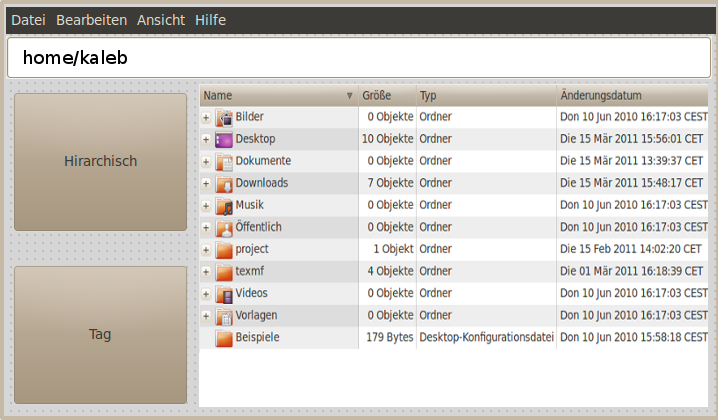
\includegraphics[scale=0.6]{ansicht1.png}
   \caption{Programm im Modus zur hierarchischen Ansicht}
\end{figure}
\subsection{Tag-Ansicht}
\begin{figure}[h!]
    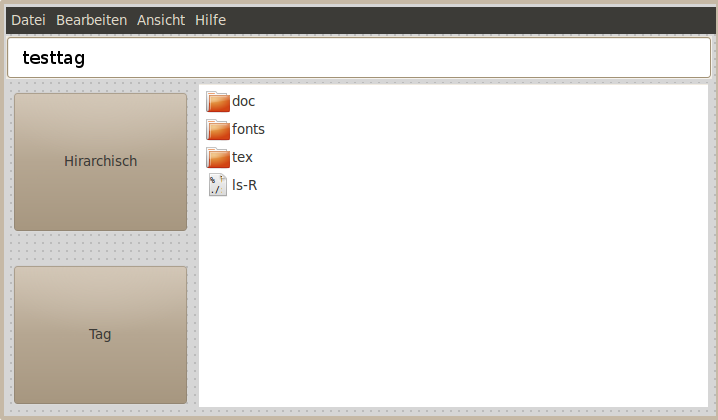
\includegraphics[scale=0.6]{ansicht2.png}
   \caption{Programm im Modus zur Ansicht der Tags}
\end{figure}
\newpage
\subsection{Tags mit Datei verkn\"upfen}
\begin{figure}[h!]
    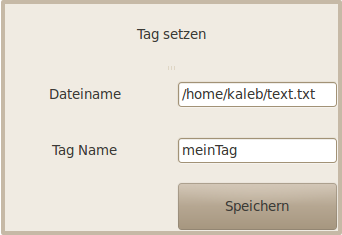
\includegraphics[scale=0.6]{vk1.png}
   \caption{Einer Datei Tags zuweisen}
\end{figure}
\subsection{Tags einer Datei \"andern}
\begin{figure}[h!]
    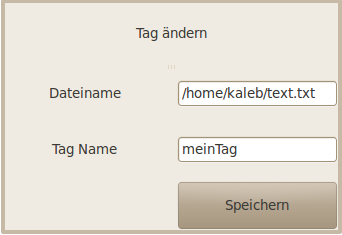
\includegraphics[scale=0.6]{vk2.png}
   \caption{Die einer Datei zugewiesenen Tags bearbeiten}
\end{figure}
\newpage
\section{Systemarchitektur}
\subsection{Gliederung der L\"osung in Module}
\begin{figure}[h!]
    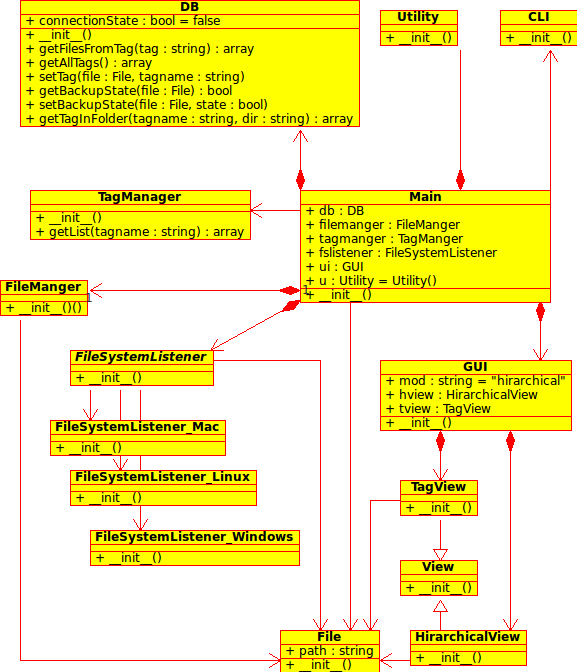
\includegraphics[scale=1.0]{diag1.png}
   \caption{Entwurf des Klassendiagrammes}
\end{figure}
Die Klasse DB dient als Schnittstelle zur Datenbank und damit zum Datenmodell, wie unten aufgezeigt.\\
Eine Instanz der Klasse File repr\"asentiert jeweils eine virtuelle oder reale Datei auf dem Dateisystem und dient als entsprechender Informationstr\"ager innerhalb der Applikation.
\subsection{Schnittstellen}
\begin{enumerate}
  \item Interne Schnittstellen ergeben sich aus dem Klassendiagramm.
  \item Externe Schnittstellen:
    \begin{enumerate}
      \item Für den normalen Gebrauch haben wie das GUI. Beim GUI wird Wert auf das einfache verwalten von Tags und Dateien gelegt.
	\begin{enumerate}
	  \item Das GUI bietet zwei Modi, einer der den herkömlichen Dateimanagern mit hierarchischer Ansicht entspricht und
	  \item Einen Tagmodus, in dem sich Dateien anhand deren Tags durchsuchen und ordnen lassen.
	\end{enumerate}
      \item Für scripting oder für solche Systeme ohne grafische Ausgabe haben wir eine CLI Version. Es wird besonders Wert auf das einfache Aufrufen von anderen Programmen (Scripts) gelegt.
	\begin{enumerate}
	  \item Die Kommandos sollen in der Bedienung weitgehend mit dem standard Unix-Tools kompatibel sein (gleiche Parameternamen für gleiche Funktionen).
	\end{enumerate}
    \end{enumerate}
\end{enumerate}
\section{Datenmodell (grob)}
\begin{figure}[h!]
    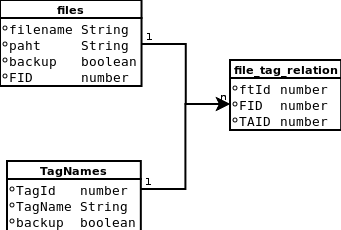
\includegraphics[scale=1.0]{diag2.png}
   \caption{Datenmodell. Stellt die DB-Struktur dar.}
\end{figure}
\section{Anforderungszuordnung}
\begin{enumerate}
  \item Main
  \item DB
  \item Utility
  \item CLI
  \item TagManager
  \item FileManager
  \item FileSystemListener
  \item GUI
  \item TagView
  \item HierarchicalView
  \item View
  \item File
\end{enumerate}
\begin{tabularx}{\textwidth}{|c|X|c|c|c|c|c|c|c|c|c|c|c|c|}
  \hline
  \bf Nr. & \bf Anforderungen &\bf 1 &\bf 2 &\bf 3 &\bf 4 &\bf 5 &\bf 6 &\bf 7 &\bf 8 &\bf 9 &\bf 10 &\bf 11 &\bf 12 \\ \hline
  1 & Das Programm starten & \cellcolor[gray]{0.7} & & & & & & & & & & & \\ \hline
  2 & GUI vorhanden & & & & & & & & \cellcolor[gray]{0.7} &\cellcolor[gray]{0.7} &\cellcolor[gray]{0.7} &\cellcolor[gray]{0.7} & \\ \hline
  3 & CLI vorhanden & & & &\cellcolor[gray]{0.7} & & & & & & & & \\ \hline
  4 & Tag hinzuf\"ugen & & & &\cellcolor[gray]{0.7} &\cellcolor[gray]{0.7} & & & &\cellcolor[gray]{0.7} & & & \\ \hline
  5 & Datei ausw\"ahlen & & & & & & \cellcolor[gray]{0.7} & & & & & & \cellcolor[gray]{0.7} \\ \hline
  6 & Versionierung & & \cellcolor[gray]{0.7} & & & & \cellcolor[gray]{0.7} & \cellcolor[gray]{0.7} & & & & & \cellcolor[gray]{0.7} \\ \hline
  7 & GUI: Versionierung f\"ur Tags & & & & & & & & \cellcolor[gray]{0.7} & & & & \\ \hline
  8 & Datei\"anderungen werden erkannt & & & & & & & & \cellcolor[gray]{0.7} & & & & \\ \hline
  9 & L\"oschen wird erkannt & & & & & & & & \cellcolor[gray]{0.7} & & & & \\ \hline
  10 & Neue Dateien werden erkannt & & & & & & & & \cellcolor[gray]{0.7} & & & & \\ \hline
  11 & Hierarchische Anzeige & & & & & & & & & & & \cellcolor[gray]{0.7} & \\ \hline
  12 & Tag Anzeige & & & & & & & & & \cellcolor[gray]{0.7} & & & \\ \hline
\end{tabularx}
\section{Mittelbedarf}
\begin{itemize}
  \item Sachmittel
    \begin{itemize}
      \item Programmierumgebung
      \item Internetzugang
    \end{itemize}
  \item Personal
    \begin{itemize}
      \item Das Personal ist durch das Projekt vorgegeben.
      \item Wir benötigen einen Projektleiter.
      \item Da der Programmieraufwand aber recht gross ist, brauchen wir neben den zwei Vollzeiprogrammierern muss auch der Projektleiter nebenbei als Entwickler tätig sein.
    \end{itemize}
  \item Ausbildung
    \begin{itemize}
      \item Einige der Programmierer werden Python lernen müssen.
    \end{itemize}
  \item Dienstleistungen
    \begin{itemize}
	\item SVN Repository
	\item Wiki
	\item Kommunikation (Email)
    \end{itemize}
\end{itemize}
\section{Planung und Organisation}
\begin{itemize}
  \item erforderliches Projektteam (Zusammensetzung, Mitwirkung der Fachabteilungen)
  \item Meilensteine
\end{itemize}
\section{Wirtschaftlichkeit}
\begin{itemize}
  \item Nutzen abschätzen
    \begin{itemize}
      \item Der Nutzer ist sehr gross, weil man sich viel weniger mit dem Dateiverwalten ausseinandersetzen muss.
    \end{itemize}
  \item Kosten abschätzen
    \begin{itemize}
      \item Da wir eine kostenlose Programmiersprache und und Google Code verwenden haben wir keine direkte Kosten.
    \end{itemize}
  \item Nutzen und Kosten gegenüberstellen
    \begin{itemize}
      \item Grosser Nutzen und keine Kosten: Es lohnt sich.
    \end{itemize}
\end{itemize}
\section{Konsequenzen}
\begin{description}
  \item{\bf Auswirkungen (organisatorisch, personell, baulich, Vorschriften/Weisungen)} \\ Es stehen neue Wege zum Organisieren und Finden von Dateien zur Verfuegung.
    Das Organisieren von Projekten die sich ueber mehrere Ordner verteilen wird vereinfacht.
    Die Beteiligten sammeln Erfahrungen mit den im Projekt eingesetzten Technologien.
  \item{\bf bei Nichtrealisierung} \\ Schlechte Note.
  \item{\bf bei verspäteter Realisierung (gegenüber Wunschtermin)} \\ Schlechte Note
  \item{\bf auf Schnitts.tellen zu anderen Systemen} \\ Das Programm ist f\"ur den lokalen offline Einsatz vorgesehen. Onlinemodul falls wir genug Zeit haben.
  \item{\bf Qualitätsverbesserungen} \\ Einfacherer Umgang mit Dateien. Mehr Moeglichkeiten zur Verwaltung von Dateien auf dem lokalen Betriebssystem.
  \item{\bf Risikobeurteilung} \\ Da das Team viel neues lernen muss und das Projekt recht viele einzelne Teile beinhaltet ist das Risiko, dass es nicht gaenzlich fertiggestellt werden kann als beachtlich einzustufen.
    Wenn das Programm keine Vorteile gegenüber anderen Dateiverwaltungstools beinhaltet, gerät das Programm in Vergessenheit.
  \item{\bf Ausweichmöglichkeiten} Herkoemmliche Dateimanager (Die ohnehin unschlagbaren tools ls,cp,rsync,mv,rm,find,locate).
\end{description}
\section{Antrag auf Freigabe der nächsten Projektphase}
Wir bitten Sie um die Freigabe der nächsten Projektphase.
\end{document}
